\begin{tcolorbox}
Die Produktfunktionen beschreiben jede einzelne Funktion des Produkts mittels Anwendungsfalldiagrammen und Anwendungsfalltabellen.
Diese sollen möglichst ausschlaggebend für das zu entwickelnde System sein und nicht simple Produktfunktionen wie z.B. Login, Account erstellen, Gruppe beitreten, Passwort ändern oder ähnliches zeigen.
\autoref{fig:anwendungsfall-app-tabelle-xx-1} stellt eine exemplarische Tabelle für die Beschreibung eines Anwendungsfalls dar. Stil und Formatierung sind variabel. Nicht jede Zelle muss immer gefüllt sein.
\\\\
In  Tabelle~\autoref{fig:akteur-tabelle} werden alle auftretenden Akteure beschrieben.


\end{tcolorbox}

\begin{figure}[h]
	\centering

	\begin{tabularx}{\textwidth}{ p{.2\textwidth} | p{.2\textwidth} | X }
		\textbf{Akteur} & \textbf{Beschreibung} & \textbf{Verwendet in Anwendungsszenario} \\ \hline
		Informatiker & Programmiert tolle Sachen & Programmieren, Kaffee trinken, Schlafen \\ \hline
		NutzerIn & Anwender der web Applikation & Komposition-\{bearbeiten, erstellen, darstellen \}, Dienst einfügen
	\end{tabularx}

	\caption{Beschreibung der Akteure}
	\label{fig:akteur-tabelle}
\end{figure}


%%%%%%%%%%%%%%%
%% Anwendungsfall 1 %%
%%%%%%%%%%%%%%%

\section{Anwendungsfalldiagramm - App}

\begin{figure}[h]
	\centering
	\missingfigure{Anwendungsfalldiagramm - App}
	\caption{Anwendungsfalldiagramm - App}
	\label{fig:anwendungsfalldiagramm-app}
\end{figure}

\newpage

\begin{figure}[h]
	\centering
	\begin{tabularx}{\textwidth}{ X | X }
		\textbf{Anwendungsfall ID} & XX-1 \\ \hline
		\textbf{Anwendungsfallname} & Hier steht ein Name. \\ \hline
		\textbf{Initiierender Akteur} & Informatiker \\ \hline
		\textbf{Weitere Akteure} & Designer, Techniker  \\ \hline
		\textbf{Kurzbeschreibung} & Hier steht eine Kurzbeschreibung.  \\ \hline
		\textbf{Vorbedingungen} & -  \\ \hline
		\textbf{Nachbedingungen} & Y trifft zu.  \\ \hline
		\textbf{Ablauf} &
			\begin{enumerate}
				\item Erster ganzer Satz.
				\item Zweiter ganzer Satz.
			\end{enumerate} \\ \hline
		\textbf{Alternative} &
				\begin{enumerate}
					\item Erster ganzer Satz.
					\item Zweiter ganzer Satz.
				\end{enumerate}  \\ \hline
		\textbf{Ausnahme} &
				\begin{enumerate}
					\item Erster ganzer Satz.
					\item Zweiter ganzer Satz.
				\end{enumerate}  \\ \hline
		\textbf{Benutzte Anwendungsfälle} & YY-1 (oder Name) \\ \hline
		\textbf{Spezielle Anforderungen} & - \\ \hline
		\textbf{Annahmen} & -
	\end{tabularx}
	\caption{Anwendungsfall XX-1}
	\label{fig:anwendungsfall-app-tabelle-xx-1}
\end{figure}

\newpage


%%%%%%%%%%%%%%%
%% Anwendungsfall 2 %%
%%%%%%%%%%%%%%%

\section{Anwendungsfalldiagramm - Server}

\begin{figure}[h]
	\centering
	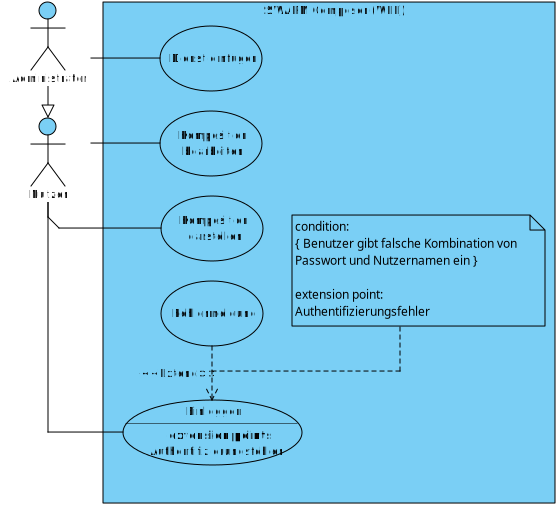
\includegraphics[width=\textwidth]{img/Produktfunktionen_web}
	\caption{Anwendungsfalldiagramm - Server}
	\label{fig:anwendungsfalldiagramm-server}
\end{figure}

\newpage

\begin{figure}[h]
	\centering
	\begin{tabularx}{\textwidth}{ X | X }
		\textbf{Anwendungsfall ID} & WEB-1 \\ \hline
		\textbf{Anwendungsfallname} & Dienst einfügen. \\ \hline
		\textbf{Initiierender Akteur} & NutzerIn \\ \hline
		\textbf{Weitere Akteure} & - \\ \hline
		\textbf{Kurzbeschreibung} & Ein neuer Dienst wird in die Datenbank eingefügt \\ \hline
		\textbf{Vorbedingungen} &   NutzerIn besitzt nötige Rechte und befindet sich auf Startseite \\ \hline
		\textbf{Nachbedingungen} & Neuer Dienst wurde in Datenbank gespeichert \\ \hline
		\textbf{Ablauf} &
		\begin{enumerate}
			\item  NutzerIn öffnet Dienst einfügen Seite.
			\item  NutzerIn gibt Dienstdetails in Eingabemaske ein.
			\item  NutzerIn bestätigt seine Eingabe.
			\item  System akzeptiert Eingabe und speichert in Datenbank.
			\item  Weiterleitung zur Hauptseite.
		\end{enumerate} \\ \hline
		\textbf{Alternative} & - \\ \hline
		\textbf{Ausnahme} &
		\begin{enumerate}
			\item  NutzerIn öffnet Dienst einfügen Seite.
			\item  NutzerIn gibt Dienstdetails in Eingabemaske ein.
			\item  NutzerIn bestätigt seine Eingabe.
			\item  System akzeptiert Eingabe nicht, da ungültige Eingabe.
			\item  System zeigt Fehler und markiert fehlende Felder.
			\item  bleibe in der Eingabemaske.
		\end{enumerate}  \\ \hline
		\textbf{Benutzte Anwendungsfälle} & - \\ \hline
		\textbf{Spezielle Anforderungen} & - \\ \hline
		\textbf{Annahmen} & Dienst erstellen Button wird nur gezeigt, falls nötige Rechte vorhanden sind.
	\end{tabularx}
	\caption{Anwendungsfall WEB-1}
	\label{fig:anwendungsfall-server-tabelle-web-1}
\end{figure}

\begin{figure}[h]
	\centering
	\begin{tabularx}{\textwidth}{ X | X }
		\textbf{Anwendungsfall ID} & WEB-2 \\ \hline
		\textbf{Anwendungsfallname} & Neue Komposition erstellen. \\ \hline
		\textbf{Initiierender Akteur} & NutzerIn \\ \hline
		\textbf{Weitere Akteure} & - \\ \hline
		\textbf{Kurzbeschreibung} & Ein neuer Dienst wird in die Datenbank eingefügt \\ \hline
		\textbf{Vorbedingungen} & NutzerIn befindet sich auf der Startseite  \\ \hline
		\textbf{Nachbedingungen} & NutzerIn befindet sich im Bearbeitungsmodus \\ \hline
		\textbf{Ablauf} &
		\begin{enumerate}
			\item  NutzerIn wählt "Komposition erstellen" Option.
			\item  NutzerIn gibt einen Namen ein.
			\item  NutzerIn wird weitergeleitet zu "Komposition bearbeiten".
		\end{enumerate} \\ \hline
		\textbf{Alternative} & - \\ \hline
		\textbf{Ausnahme} & - \\ \hline
		\textbf{Benutzte Anwendungsfälle} & WEB-3 \\ \hline
		\textbf{Spezielle Anforderungen} & - \\ \hline
		\textbf{Annahmen} & -
	\end{tabularx}
	\caption{Anwendungsfall WEB-2}
	\label{fig:anwendungsfall-server-tabelle-web-2}
\end{figure}

\begin{figure}[h]
	\centering
	\begin{tabularx}{\textwidth}{ X | X }
		\textbf{Anwendungsfall ID} & WEB-3 \\ \hline
		\textbf{Anwendungsfallname} & Komposition bearbeiten. \\ \hline
		\textbf{Initiierender Akteur} & NutzerIn \\ \hline
		\textbf{Weitere Akteure} & - \\ \hline
		\textbf{Kurzbeschreibung} & NutzerIn bearbeitet Komposition \\ \hline
		\textbf{Vorbedingungen} & NutzerIn besitzt nötige Rechte zur Bearbeitung der Komposition und befindet sich auf der Startseite \\ \hline
		\textbf{Nachbedingungen} & NutzerIn befindet sich im Bearbeitungsmodus \\ \hline
		\textbf{Ablauf} &
		\begin{enumerate}
			\item  NutzerIn drückt Bearbeitungsbutton der Komposition.
			\item  NutzerIn wird in den Bearbeitungsmodus versetzt.
		\end{enumerate} \\ \hline
		\textbf{Alternative} & - \\ \hline
		\textbf{Ausnahme} & - \\ \hline
		\textbf{Benutzte Anwendungsfälle} & - \\ \hline
		\textbf{Spezielle Anforderungen} & - \\ \hline
		\textbf{Annahmen} & Es werden nur Komposition gezeigt für die der NutzerIn die benötigten Rechte besitzt.
                  Der Bearbeitungsbutton ist ausgegraut falls die Bearbeitungsrechte nicht vorhanden sind.
	\end{tabularx}
	\caption{Anwendungsfall WEB-3}
	\label{fig:anwendungsfall-server-tabelle-web-3}
\end{figure}

\begin{figure}[h]
	\centering
	\begin{tabularx}{\textwidth}{ X | X }
		\textbf{Anwendungsfall ID} & WEB-4 \\ \hline
		\textbf{Anwendungsfallname} & Komposition darstellen. \\ \hline
		\textbf{Initiierender Akteur} & NutzerIn \\ \hline
		\textbf{Weitere Akteure} & - \\ \hline
		\textbf{Kurzbeschreibung} & NutzerIn lässt sich Komposition anzeigen \\ \hline
		\textbf{Vorbedingungen} & NutzerIn besitzt nötige Rechte zur Darstellung der Komposition und befindet sich auf der Startseite \\ \hline
		\textbf{Nachbedingungen} & NutzerIn wird Komposition dargestellt \\ \hline
		\textbf{Ablauf} &
		\begin{enumerate}
			\item  NutzerIn drückt auf die anzuzeigende Komposition.
			\item  NutzerIn wird die Komposition angezeigt.
		\end{enumerate} \\ \hline
		\textbf{Alternative} & - \\ \hline
		\textbf{Ausnahme} & - \\ \hline
		\textbf{Benutzte Anwendungsfälle} & - \\ \hline
		\textbf{Spezielle Anforderungen} & - \\ \hline
		\textbf{Annahmen} & Es werden nur Komposition gezeigt für die der Nutzer die benötigten Rechte besitzt.
	\end{tabularx}
	\caption{Anwendungsfall WEB-4}
	\label{fig:anwendungsfall-server-tabelle-web-4}
\end{figure}